%\section{Muonium hyperfine splitting measurement at J-PARC}
\section{Muonium hyperfine structure measurement}

Muonium is a hydrogen-like atom made of a positive muon and
an electron.  High precision measurements of the muonium ground
state hyperfine structure (HFS) is one of the most sensitive
test for bound state quantum electrodynamics (QED), and for
determining precisely fundamental constants of the muon magnetic
moment and hence its mass.  Indeed, hydrogen HFS is the most
precisely measured value with a precision 0.2 ppt \cite{Essen-1973},
but the theoretical value is presently limited at
0.6 ppm \cite{Eides:1012805} due to the proton internal structure.
In addition, the hyperfine structure of positronium, which
is a bound state of a positron and an electron, is limited
experimentally by its mean lifetime (i.e. 140 ns for
ortho-positronium) with an accuracy of only
3.3 ppm \cite{Ritter-etal, Mills, Ishida-etal-PLB734-338-2014},
while its theoretical value is calculated at
a level of 1.1 ppm \cite{Baker-etal-PRL.112.120407} with
uncertainties from unknown nonlogarithmic
higher-order terms.  However, lifetime of the muonium (2.2 $\mu$s)
is long enough to precisely measure hyperfine structure, and
due to its constituents have an no internal structure (pure
leptonic system), hyperfine structure can be accurately calculated.
The previous muonium HFS measurement at zero field \cite{Casperson-etal}
reached a precision of 310 ppb, while the one at high 
field \cite{Liu:1999iz} achieved
12 ppb, both performed at LAMPF and with experimental uncertainties
mostly dominated by statistical errors.  The current theoretical
value of muonium HFS is 61 ppb \cite{CODATA}, but it is reported
that effort to reach 10 ppb level is in progress.

In addition to test QED, it should be noted that the experimental
values of the muon magnetic moment and mass are currently determined
by the previous muonium HFS experiment at high
field \cite{Liu:1999iz}.  The
magnetic moment ratio between muon and proton is of the utmost
importance in the determination of the muon anomalous magnetic
moment, also called muon $g-2$, and being regarded as a keystone
at unravelling the physics of the standard model and 
beyond \cite{Otani-JPARCSympo-2015}.
Furthermore, precision microwave spectroscopy of muonium can
also contribute to many new physics such as testing CPT and
Lorentz invariance incorporated in extensions to the standard
model \cite{Hughes-etal-inBook, KosteleckyVargas-PRD92.056002},
disentangling the proton radius puzzle \cite{Pohl-etal-nature,
Brodsky-etal-PRL94.022001},
searching for exotic particle \cite{Karshenboim-PRL104.220406,
KarshenboimFlambaum-PRA84-2011}, and even probing for
long-range neutrino-mediated forces \cite{Stadnik}.

The MuSEUM collaboration is now planning new and complementary
measurements of the muonium HFS both at zero field and at a high
magnetic field of 1.7 T.  Our goal is to improve the precision
of these measurements by one order of magnitude.  The new
high-intensity surface muon beamline, H-Line, that will soon be
available at J-PARC MUSE \cite{Higemoto-etal}, will provide
an opportunity to achieve that goal.

However, as we improve the statistics, understanding and suppressing
systematic uncertainty become essential.  Developments were performed
and tools have been created to suppress uncertainties associated
with the magnetic field inhomogeneity, muon stopping distribution,
microwave power fluctuation and gas density extrapolation.  An
overview of the different aspects of these new precise muonium
HFS measurements, the current status of the preparation for
high-field measurements, and the latest measurements at zero
field are presented.


The muonium hyperfine is measured by the spectroscopy of the
spin states.  The Hamiltonian of the ground state muonium is
expressed as
%
\begin{align}
 H  =    h \nu_{\text{HFS}} \mathbf{s}_\mu \cdot \mathbf{s}_e
      - \mu_\mu g'_\mu \mathbf{s}_\mu \cdot \mathbf{H} 
      + \mu_e g'_e \mathbf{s}_e \cdot \mathbf{H} 
\end{align}
%
where $\nu_{\text{HFS}}$ is the muonium hyperfine structure,
$\mu_\mu$ ($\mu_e$) is the magnetic moment, $g'_\mu$ ($g'_e$)
is the bound $g$-factor of muon and electron in the muonium,
and $\mathbf{s}_\mu$ ($\mathbf{s}_e$) is the spin of the muon
(electron).  The muonium hyperfine structure is measured by
the measurement at $\mathbf{H}=0$ by measuring the energy level
between the spin singlet and triplet.  When $\mathbf{H}$
is non-zero, the spin triplet split to three sublevels, which
is called the Zeeman effect.  Figure \ref{fig:BreitRabi} shows
the Breit Rabi diagram of the muonium 1S$_{1/2}$ state.

\begin{figure}[th]
 \centering
 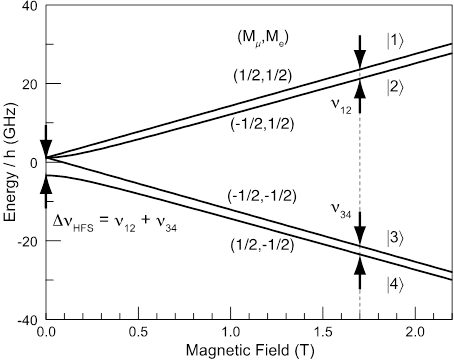
\includegraphics[width=0.5\textwidth, bb= 0 0 227 181]
                 {./Fig/MuHFS-BreitRabi.png}
\caption{\label{fig:BreitRabi}
Breit-Rabi energy level diagram for muonium atom under magnetic field.}
\end{figure}

In the MuHFS measurement with high magnetic field,magnetic
moment ratio of muon and proton can be derived from the
transition frequencies between the Zeeman sublevels $\nu_{12}$
and $\nu_{34}$ which are expressed as 
%
\begin{align}
\nu_{12}&= \frac{\mu_\mu g'_\mu H}{h}
           + \frac{\nu_{\text{HFS}}}{2}
             \left[ (1+x) - \sqrt{1+x^2} \right]~,\\
\nu_{34}&= \frac{\mu_\mu g'_\mu H}{h}
           + \frac{\nu_{\text{HFS}}}{2}
             \left[ (1+x) + \sqrt{1+x^2} \right]~,
\end{align}
%
where $x=\frac{(g'_e \mu_e + g'_\mu \mu_\mu)H}{h\nu_{\text{HFS}}}$.
The magnetic field $H$ can be measured with the nuclear magnetic
resonance (NMR) precession frequency of free proton $\mu_p$
as $h\nu_p = 2\mu_p H$.  Therefore, the muonium hyperfine
structure can be measured by $\nu_{\text{HFS}}=\nu_{12}+\nu_{34}$
and also the muon to proton magnetic moment ratio is derived
by $\nu_{12}, \nu_{34}$ and $\nu_p$.  This value is measured
at LAMPF with 120 ppb precision as $\mu_\mu/\mu_p =
3.183 \, 345  \, 24(37)$.  This measurement is also used to
determine the values of the muon to electron mass ratio.
%
\begin{align}
\frac{m_\mu}{m_e}
=
\left( \frac{g_\mu}{g_e} \right)
\left( \frac{\mu_\mu}{\mu_p} \right)^{-1}
\left( \frac{\mu_e}{\mu_p} \right) ~.
\end{align}
%
As the major uncertainty of this formula is caused by
$\mu_\mu/\mu_p$, therefore the precision of the muon-electron
mass ratio is determined as $m_\mu/m_e= 206.768 \, 276(24)$ (120ppb).
$m_\mu/m_e$ is also measured in other methods.for example, the
muonium 1S-2S interval measurement by the Doppler-free two-photon
laser spectroscopy, $m_\mu/m_e$ was extracted as $206.768 \, 38(17)$
\cite{Meyer-etal-PRL84.1136}.  By combining other experimental
results and comparing to the theoretical prediction, we can
have a stringent test of the bound state QED also with $m_\mu/m_e$.


\begin{figure}[th]
 \centering
 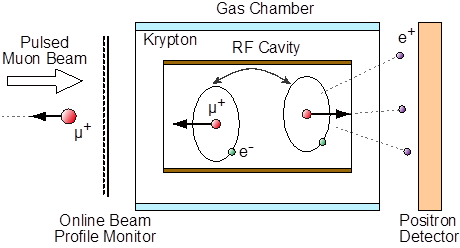
\includegraphics[width=0.7\textwidth, bb=0 0 230 124]
                 {./Fig/MuHFS-MuSEUM-setup.png}
\caption{\label{fig:MuSEUM-setup}
Schematic view of the experimental setup.  This apparatus is
either enclosed in a magnetic shield box for zero-field
measurements, or inserted in a large superconducting solenoid
magnet for high-field measurements.}
\end{figure}

The schematic view of the experimental setup is shown in
Fig.~\ref{fig:MuSEUM-setup}, and the experimental procedure
can be summarized as follows: (1) muonium formation, (2) RF
spin flip, and (3) positron asymmetry measurement.  High-intensity
pulsed muon ($\mu^+$) beam, 100\% backward polarized with
respect of the muon momentum direction, are injected into
a RF cavity located inside a gas chamber containing highly
pure krypton gas.  The profile of the incident muon beam
is measured online by a non-destructive beam profile monitor
located in front of the entrance window of the gas chamber.
The $\mu^+$ are stopped in Kr gas and rapidly form polarized
muonium atom through a charge exchange reaction with Kr atoms.
The muon spin can be flipped by applying a microwave magnetic
field in the RF cavity perpendicular to the muon direction.
The positrons ($e^+$) from muon decay are emitted preferentially
in the direction of the muon spin.  At the resonance, the
RF field induces the muon spin flip changing the angular
distribution of the emitted positrons from primarily backward
to forward direction.  Positrons are then detected with
segmented scintillation detectors placed downstream of the
gas chamber.  Muonium spectroscopy is then performed by
scanning the RF frequency and measuring positrons to determine
resonance frequencies. i.e., $\Delta \nu_{\text{HFS}}$
at zero field and $\nu_{12}$ and $\nu_{34}$ at high field,
respectively.


For zero-field measurements, the apparatus is enclosed in a
magnetic shield box made of three layers of permalloy to
suppress residual magnetic field.  The experiment will be
performed at the existing D-Line of the MUSE facility at
J-PARC \cite{Higemoto-etal}.  For high-field measurements,
a large superconducting solenoid with an applied static field
of 1.7 T parallel to the muon momentum direction will be used.
This static magnetic field and the introduced RF field in
the cavity, perpendicular to the solenoid field, splits the
ground state of the muonium into the four different substates
as shown in Fig.~\ref{fig:BreitRabi}.  The high-intensity
surface muon beam with an expected intensity of 
$1\times 10^{8} \mu^+/{\text{s}}$ will be provided by the new
H-Line that is under construction at J-PARC MUSE.

The progress of these new muonium HFS measurements are being
reported regularly.  The latest publications can be found
in Refs.~\cite{Strasser2016, Ueno2017,
Shimomura-etal-doi:10.1142/9789813148505_0008,
T.Tanaka-etal-PSAS2018}.  Here a brief overview of the different
aspects of this experiment is presented focusing mainly on
the recent developments: preparation for high-field measurements,
latest measurements at zero field,and development of the time
differential method.  Several types of detectors are being
used in these measurements.  First, an online fiber beam
profile monitor measures the muon beam pulse by pulse to
suppress systematic uncertainty related to the muon beam
profile and intensity stability \cite{Kanda-PhotoDet2015}.
Second, a 3D muon
beam monitoring system was used offline to measure the muon
beam stopping position in the Kr gas chamber at various gas
pressure to reduce systematic uncertainty related to muonium
atom distribution \cite{Ueno2017, Y.Ueno-etal-LEAP2016}.
Finally, an integrated highly-segmented
scintillation detector system with high-rate capability is
used to detect positrons \cite{Kanda-PhotoDet2015,
Kanda-etal-JPARCSympo2015}.


Recently, a new type of positron detector made of a highly-segmented
silicon strip sensor with high-rate capability is being developed
and tested \cite{Nishimura-phdthesis}.  
Figure \ref{fig:MuSEUM-IntegratedSiliconStripDetector}
shows a picture of this new integrated silicon strip detector.
The silicon strip sensor has an active area of 97.28 mm square
divided in two blocks with a thickness of 0.32 mm.  The strip
pitch and length are 0.19 mm and 48.575 mm, respectively.
The number of strips is $512 \times 2$ blocks.  The silicon
strip sensor is connected on both sides though an adapter
to two multi-Slit128A boards, where signals are directly
processed by an analog/digital combined type integrated circuit.
Each board contains four readout SliT128A chips, ASIC-based
(Application Specific Integrated Circuit) ASD
(amplifier-shaper-digitizer), that are controlled by an FPGA
(Field Programmable Gated Arrays).  This silicon strip detector
was originally developed for J-PARC $g-2$/EDM
experiment \cite{Otani-JPARCSympo-2015}.
Details and performance of this new positron detector will be
reported soon elsewhere.
   

\begin{figure}[th]
 \centering
 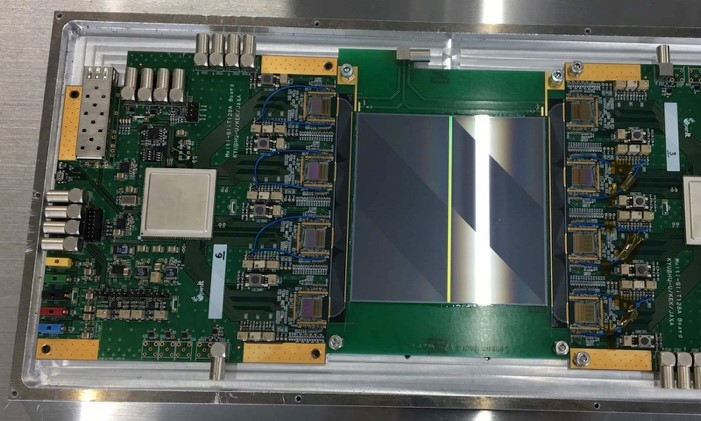
\includegraphics[width=0.7\textwidth, bb=0 0 229 138]
                 {./Fig/MuHFS-IntegratedSiliconStripDetector.jpg}
\caption{\label{fig:MuSEUM-IntegratedSiliconStripDetector}
Integrated silicon strip detector.  The sensor is directly
connected on both sides to an analog/digital combined type
integrated circuit for readout and signal processing through
four ASIC-ASDs (Slit128A) controlled by a FPGA.}
\end{figure}

High-field measurements will be performed with a superconducting
solenoid magnet that was recycled from an old MRI magnet designed
for high homogeneous magnetic field.The choice of a longer cavity
to allow measurement at lower Kr gas density imposes strict
requirements on the magnet.  Indeed, the systematic uncertainty
on the magnetic field was the second largest uncertainty in
the previous experiment at LAMPF \cite{Liu:1999iz}.  
The muonium HFS frequency
$\Delta \nu_{\text{HFS}} (=\nu_{12}+\nu_{34})$ is in principle
independent of the magnetic field.  However, $\mu_\mu/\mu_p$
($=\nu_{34}- \nu_{12}$) is dependent on the magnetic field, 
and its inhomogeneity relates largely to the systematic
uncertainty.  But since both $\nu_{12}$ and $\nu_{34}$ are
measured separately, a precise calibration is still required
in both cases.  The present requirements for the magnetic
field are a homogeneity of $<1$ ppm with absolute calibration
in a spheroidal volume of $\phi 200$ mm $\times$ 300 mm
(muon stopping region), a field stability of 0.1 ppm/h,
and an absolute calibration at 10 ppb level.  Improvement
of the homogeneity of the MRI magnet and development of NMR
probes for absolute magnetic field calibration is steadily
progressing.


Commissioning test of the MRI magnet was performed.After several
iterative shimming processes, a field homogeneity within 0.8
ppm peak-to-peak in the muon stopping spheroid was reached.
The long-term stability was measured at 3 ppb/hour over a 10
days period.  The helium evaporation rate was 3 L/day.  All
this fulfills our design values.

For the precise magnetic field monitoring,a continuous wave
NMR (CW-NMR) system with a RF pickup coil is being developed
for both $g-2$/EDM and MuSEUM experiments at J-PARC.  A field
mapping probe with 24 RF pickup coils is being constructed
to scan the muon stopping spheroid inside the MRI magnet.
Also, a cross calibration test is in progress at Argonne
National Laboratory with the pulse-NMR probe used at the
FermiLab muon storage ring experiment \cite{Bennett:2006fi}.
The magnetic field is measured at the same position by both
probes.  The development of the CW-NMR probe is reported in
details in \cite{T.Tanaka-etal-PSAS2018}.  Preliminary
measurements showed that a resolution of 18 ppb could be
reached \cite{Sasaki-etal-IEEE}.  Recently, even better
resolution was obtained, but the analysis is still in progress
and the results will be published elsewhere.


Commissioning test experiments at zero field are being performed
since February 2016 at the D2 experimental area (D-Line) of
the MUSE facility.  These engineering runs are crucial to test
the different aspects of the apparatus and grasp possible
problems to be overcome before the start of the high-field
measurements.  Zero-field measurements are also important
because of different systematics from the magnetic field
(negligible at zero field).  Figure \ref{fig:MuSEUM-ZeroFieldExp-setup}
shows the apparatus during one of the engineering runs.  
The residual magnetic field is suppressed below 100 nT
by a magnetic shield made of three layers of 1.5-mm thick
permalloy that enclose completely the gas chamber and RF cavity.

\begin{figure}
 \centering
\begin{overpic}[width=0.7\textwidth,bb=0 0 701 525]
                 {./Fig/image017.jpg}
\put(0,-3.5){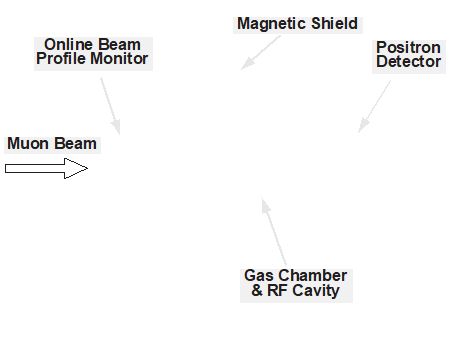
\includegraphics[width=0.75\textwidth, bb=0 0 227 170]
{./Fig/MuHFS-MuSEUM-ZeroFieldExp-setup.png}}
\end{overpic}
\caption{\label{fig:MuSEUM-ZeroFieldExp-setup}
Experimental setup for zero-field measurements at area D2 of MUSE D-Line.
}
\end{figure}


Since the first resonance peak was observed in June 2016,
systematic uncertainties due to gas pressure and impurity,
RF power stability and muon beam profile distribution were
studied.  As we improve the statistics, the systematic uncertainty
becomes more severe and needs to be carefully considered.
It should be noted that our understanding of the systematical
error in an experiment is limited by the time spent on the
measurements, and that longer the measurement time, the
lower the systematic uncertainty.


Figure \ref{fig:MuSEUM-MuSEUM-lineshape} shows a typical
resonance lineshape of the muonium HFS transition as a
function of the applied RF frequency detuned from 4463.3 MHz
measured in March 2018 (scintillation detector data).
The time integral method is used by measuring alternatively
RF ON and OFF at different detuning frequencies and taking
the difference, i.e., 
$(N_{\text{ON}}-N_{\text{OFF}})/N_{\text{OFF}}$.  
The blue line shows a preliminary Lorentzian fitting result.
   

\begin{figure}[th]
 \centering
 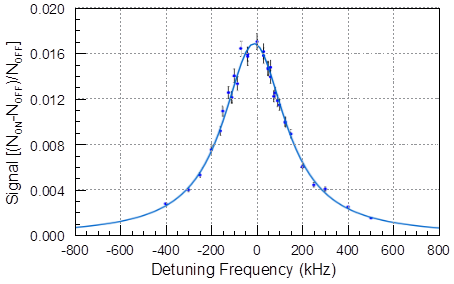
\includegraphics[width=0.7\textwidth, bb=0 0 227 142]
                 {./Fig/MuHFS-MuSEUM-lineshape.png}
\caption{\label{fig:MuSEUM-MuSEUM-lineshape}
Typical muonium HFS transition resonance lineshape as a
function of the applied RF frequency detuned from 4463.3 MHz.
The blue line shows a preliminary Lorentzian fitting result.
The data analysis is in progress.
}
\end{figure}


New precise muonium HFS measurements are important for further
QED testing and new fundamental physics experiments.  Improving
the overall accuracy, estimating and understanding systematic
uncertainties are essential in reaching that goal.  Measurements
at zero field are yielding their first results at MUSE D-Line.
Preparation for the high-field measurements at H-Line are
steadily progressing.  At present, it is unclear when the
new H-Line will be operational, but we are aiming at a first
test experiment at high field sometime in 2019-2020.



